Most of the material presented in this Section is not original, we use it mainly as
a reminder and an opportunity to present quantities and notations that will be
used later on.
We consider a system consisting of two phases, separated by a sharp interface $\Sigma(t)$ which evolves over time. 
Each phase subdomain is denoted $\Omega_1(t)$ and $\Omega_2(t)$ for the continuous phase ($1$) and the dispersed phase ($2$) respectively (see \ref{fig:Scheme}). 
The mathematical and physical definition of $\Sigma(t)$ is by no means straightforward, therefore, the interested reader is refereed to \cite{bothe2022sharp} to have a deeper understanding of sharp interface modeling. 
The entire domain, denoted as $\Omega$, is defined as the union of $\Omega_1$, $\Omega_2$, and $\Sigma$.
To track the position of the phase indexed $k$, we introduce the phase indicator function, 
\begin{equation}
    \chi_k(\textbf{y},t) =  \left\{
      \begin{tabular}{cc}
        $1 \;\text{if} \;\textbf{y} \in \Omega_k(t)$\\
        $0 \;\text{if} \;\textbf{y} \notin \Omega_k(t)$
      \end{tabular}
      \right.
      \text{for $k = 1,2$}
      \label{eq:PIF}
\end{equation}
which is null everywhere except inside the phase $k$. 
In the following, we omit the time and position arguments of $\chi_k$. 
\todo[inline]{introduce interface indicator function}
\begin{figure}[h!]
    \centering
    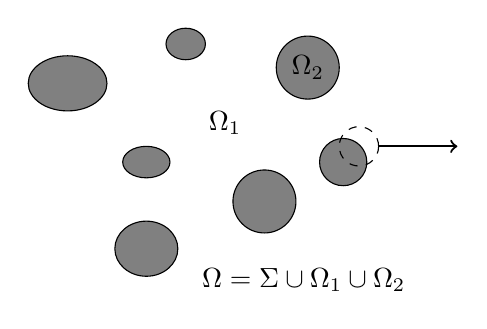
\begin{tikzpicture}
        \foreach \x/\y/\ra/\r in {
        1/3/0.2/0.25,
        2.55/2.7/0.4/0.4,
        0.5/0.4/0.35/0.4,
        2/1/0.4/0.4,
        3/1.5/0.3/0.3,
        0.5/1.5/0.2/0.3,
        -0.5/2.5/0.35/0.5}{
            \draw[fill=gray](\x,\y) ellipse(\r cm and \ra cm);
        }
        \draw[dashed](3.2,1.7)circle(0.25);
        % \draw[thick,->](3.2,1.7)++(0.1767,0.1767)--++(0.4,0.4)--++(1,0);
        \draw[thick,->](3.2,1.7)++(0.25,0)--++(1,0);
        \draw(2.55,2.7)node{$\Omega_2$};
        \draw(1.5,2)node{$\Omega_1$};
        \draw(2.5,0)node{$\Omega = \Sigma \cup \Omega_1 \cup \Omega_2$};
        % \draw(2.5,-1)node{$\Sigma = \sum_\alpha \Sigma_\alpha$};
        % \draw(2.5,-0.5)node{$\Omega_2 = \sum_\alpha \Omega_\alpha$};
    \end{tikzpicture}
    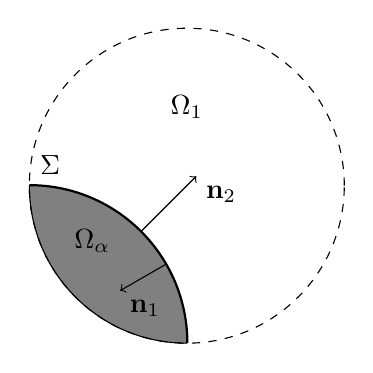
\begin{tikzpicture}%[scale = 0.9]
        \draw[very thick](0:2)arc(0:90:2)node[above right]{$\Sigma$};
        \draw[fill=gray](0:2)arc(0:90:2)arc(180:270:2);
        \draw[dashed](2,2)circle(2);
        \draw[->](1.42,1.42)--++(0.7,0.7)node[below right]{$\textbf{n}_2$};
        \draw[->](1.73,1)--++(-0.577,-0.333)node[below right]{$\textbf{n}_1$};
        \draw(2,3)node{$\Omega_1$};
        \draw(0.8,1.3)node{$\Omega_\alpha$};
    \end{tikzpicture}
    \caption{Domain definitions and scheme of the topology of dispersed two-phase flows.}
    \label{fig:Scheme}
\end{figure}

\subsection{Local conservation equations}
\label{sec:local_eq}

For the purpose of clarity, we only consider the specific case of the mass, momentum and energy conservation equations for a buoyant dispersed two phase flow.
Besides, we restrict the examples to the cases without mass transfer.

\subsubsection{Inside the volumes}
Within phase $k$, we note $\rho_k$ the density, $\textbf{u}_k^0$ the local velocity and $E_k^0$ the local total energy per units of mass.
All over the domain $\Omega_k(t)$ the mass, momentum and total energy obey these conservation laws :

\begin{align}
    \label{eq:dt_rho}
    \pddt \rho_k  
    + \div (
        \rho_k\textbf{u}_k^0
    )
    &= 
    0\\
    \label{eq:dt_rhou_k}
    \pddt (\rho_k\textbf{u}_k^0)  
    + \div (
        \rho_k\textbf{u}_k^0\textbf{u}_k^0
        - \bm{\sigma}_k^0 
    )
    &= 
    \rho_k \textbf{g}\\
    \label{eq:dt_rhoE_k}
    \pddt (\rho_kE_k^0)  
    + \div (
        \rho_kE_k^0\textbf{u}_k^0
        + \textbf{q}_k^0
        - \textbf{u}_k^0 \cdot \bm{\sigma}_k^0 
        )
    &= 
    \textbf{u}_k^0 \cdot \textbf{g}  \rho_k
\end{align} 
where $\bm{\sigma}_k^0 = - p_k^0 \textbf{I} + \bm{\tau}_k^0$ is the Newtonian stress tensor with $p_k ^0$ the local pressure and $\bm{\tau}_k^0 = \mu_k[\grad \textbf{u}_k^0+(\grad \textbf{u}_k^0)^T]$ the shear rate. 
The vector $\textbf{q}_k^0$ represent the thermal energy flux and is often model with a Fourier law : $\textbf{q}_k^0 = -\lambda \grad T_k^0$
and $\textbf{b}^0_k$  and the local body forces.

Defining $E_k^0 = e_k^0 + (u_k^0)^2/2$ where  $e_k^0$ is the internal energy which represent the molecular agitation and $(u_k^0)^2/2$ is the kinetic energy per unit of mass, leads us to two independent equation for the energy, 
\begin{align}
    \label{eq:dt_rhou_k2}
    \pddt [\rho_k(u_k^0)^2]  
    + \div [\rho_k(u_k^0)^2\textbf{u}_k^0/2 - \textbf{u}_k^0 \cdot \sigma_k^0]
    &=
    \rho_k\textbf{u}_2^0 \cdot \textbf{g}  
    -  \bm{\sigma}_k^0 : \grad \textbf{u}_k^0 
    \\
    \label{eq:dt_rhoe_k}
    \pddt (\rho_ke_k^0)  
    + \div (
        \rho_ke_k^0\textbf{u}_k^0
        + \textbf{q}_k^0
        )
    &= 
    \bm{\sigma}_k^0 : \grad \textbf{u}_k^0
\end{align} 
where, the term $\bm{\sigma}_k^0 : \grad \textbf{u}_k^0$ appears with opposite sign in both conservation equation which denote the transfer of energy across scales. 

\subsubsection{On interfaces}

The interface mass and momentum two-dimensional conservation equation which can be viewed as the jump condition at the interface are well established.
However, the energy conservation law jump condition at the interface is less employed.
Assuming no mass exchanges, i.e. the  $\textbf{u}_I^0 = \textbf{u}_k^0$ on $\Sigma(t)$ nor momentum  nor kinetic energy accumulation at the interface, the momentum and energy surface equations can be written as, 
\begin{align}
    \label{eq:dt_rhoIu_I}
    \pddt (\rho_I\textbf{u}_I^0)  
    + \divI (
    \rho_I\textbf{u}_I^0
    -\sigma \textbf{I}_{||} )
    &= 
    \rho_I \textbf{g}
    - \Jump{
        % \rho_k \textbf{u}_k (\textbf{u}_I - \textbf{u}_k)
        \mathbf{T}_k
    }\\
    \label{eq:dt_rhoIE_I}
    \pddt (\rho_I\sigma)  
    + \divI (
        \rho_I\sigma\textbf{u}_I^0
        - \textbf{u}_I^0 \cdot \bm{\sigma}_I^0 
        + \textbf{q}_{I||}^0
        )
    &= 
    \textbf{u}_k^0 \cdot \textbf{g}  \rho_I
    - \Jump{\textbf{u}_k^0 \cdot \bm{\sigma}_k^0 - \textbf{q}_k^0}
\end{align} 
We now assume that the diffusive flux of the surface is solely due to surface tension, therefore $\bm{\sigma}_I^0  = \gamma (\textbf{I} - \textbf{nn}) = \gamma \textbf{I}_{||}$ where $\gamma$ is the surface tension coefficient \citep[Chapter 2]{tryggvason2011direct}.  
Note that in a more general case, interfacial viscous stress could be included \citep{brenner2013interfacial,slattery2007interfacial} due to contamination of the interface, but it will not be addressed in this study. 
In practice, we make assume the surface density to be negligible thus $\rho_I = 0$, which simplifies the surface momentum and total energy equations to,
\begin{align}
    \Jump{\bm{\sigma}_k^0} 
    &=
    \gamma\kappa\textbf{n}
    + \gradI\sigma 
    \label{eq:surface_tension}\\
    \label{eq:dt_rhoIu2_I}
    \Jump{\textbf{u}_k^0 \cdot \bm{\sigma}_k^0}
    &= 
     \gamma\kappa\textbf{n}\cdot \textbf{u}_{I}^0\\
    \label{eq:dt_rhoIe_I}
    \Jump{ \textbf{q}_k^0}
    &= 
     0
\end{align}
\tb{true without Marangonie}
where $\kappa = - \div\textbf{n}$ is the curvature of the surface.
The decomposition of the total energy jump condition into\ref{eq:dt_rhoIu2_I} and \ref{eq:dt_rhoIe_I} has been possible thanks to the consideration of no mass transfer at the interface, in which case we have $\textbf{u}_I^0=\textbf{u}_k^0$ for $k =1,2$. 
In \ref{eq:surface_tension}, we can clearly identify two contributions : the first one related to the curvature, and the second one from the non-constant surface tension coefficient along the surface. 
The latter contribution is responsible for the Marangonie effect.
The energy jump corresponds to the work done by surface tension forces ? 

It is important to note that \ref{eq:dt_f_k} and \ref{eq:dt_f_I} are solely defined within $\Omega_k(t)$ and $\Sigma(t)$ respectively.
Consequently, these equations are referred to as local conservation equations.

\subsubsection{Generic equations}

In the following the derivation will be similar for each equation therefor it is useful to define a generic equation on which we perform the algebra.
Let $f_k^0(\textbf{y},t)$ denote a volumetric quantity of arbitrary tensorial order defined in $\Omega_k(t)$.
Likewise, let $f_I^0(\textbf{y}_I,I)$ represent an arbitrary surface property defined on $\Sigma(t)$.
Using the strategy outlined in \citep{bothe2022sharp,morel2015mathematical,slattery2007interfacial}, we can derive the local conservation equations for both $f_k^0(\textbf{y},t)$ and $f_I^0(\textbf{y}_I,t)$.
They read,  
\begin{align}
    \label{eq:dt_f_k}
    \pddt f_k^0
    +\div \left(
        f_k^0\textbf{u}_k^0
        - \mathbf{\Phi}_k^0
        \right)
    &= 
    s_k^0
    & \text{ in } \Omega_k(t),&\\
    \pddt f_I^0 
    +\divI
    (
        f_I^0 \textbf{u}_I^0
        - \mathbf{\Phi}_{I||}^0 
    )
    &= 
    s_I^0
    - \Jump{
        f_k (\textbf{u}_I^0 - \textbf{u}_k^0)
        + \mathbf{\Phi}_k^0
     } 
    & \text{ on } \Sigma(t),&
    \label{eq:dt_f_I}
\end{align}
for respectively, $f_k^0$ and $f_I^0$.
The tensors $\mathbf{\Phi}_k^0$ and $\mathbf{\Phi}_{I||}^0$ represent the non-convective fluxes corresponding to $f_k^0$ and $f_I^0$. 
Notice that $\mathbf{\Phi}_{I||}^0$ carries the $_{||}$ subscript which implies that only the tangential component of this tensor remain in the surface balance equation. 
Similarly, $s_k^0$ and $s_I^0$ represent the source terms for $f_k^0$ and $f_I^0$ respectively.
Lastly, $\textbf{u}_k^0$ corresponds to the velocity field defined in $\Omega_k(t)$, while $\textbf{u}_I^0$ corresponds to the velocity field defined on $\Sigma(t)$.
In \ref{eq:dt_f_I} we also introduced the notation $\Jump{\ldots}$, which is defined as $\Jump{\ldots} = \sum_{k=1}^2 [\ldots] \cdot \textbf{n}_k$.
This term account for the discontinuity of the flux $\left[f_k^0 (\textbf{u}_I^0 - \textbf{u}_k^0)+ \mathbf{\Phi}_k^0\right]\cdot\textbf{n}_k$ in each phases across the interfaces.
\tb{introduce the jump as the lim at each interface, look in math book too}


\subsection{Topological equations}

Using the distribution formalism, one may show that the transport equation of $\chi_k$ reads\citep{drew1983mathematical} 
\begin{equation}
    \pddt \chi_k
    + \textbf{u}_I^0 \cdot \grad \chi_k
    = 0,
    \label{eq:dt_chi_k}
\end{equation}
where $\textbf{u}_I$ is the velocity of the interface $\Sigma(t)$.
Additionally, it can be shown  \citep{drew1983mathematical} that,
\begin{equation}
    \grad \chi_k
    = - \delta_I \textbf{n}_k
    \label{eq:grad_chi_k}
\end{equation}
where we introduced the interface indicator function defined as $\delta_I = \delta(\textbf{y}-\textbf{y}_I)$ where $\delta$ is the Dirac-delta function and $\textbf{y}_I$ the position of the interface. 
Furthermore, we introduced $\textbf{n}_k$ as being the outward normal vector associated with the domain $\Omega_k$ (see \ref{fig:Scheme}).
To describe the evolution of $\delta_I$ we take the gradient of \ref{eq:dt_chi_k} which yields \citep{morel2015mathematical},
\begin{equation}
    \pddt \delta_I
    + \div \left[(\textbf{u}_I^0\cdot\textbf{n})\textbf{n} \delta_I\right]
    = \delta_I (\textbf{u}_I^0\cdot\textbf{n})(\div\textbf{n}),
\end{equation}
where we did not specify the index of \textbf{n} since it appears twice in all terms of the equation. 
As pointed out by \citet{morel2007surface}, it is more convenient to rewrite this equation under the following form,
\begin{equation}
    \pddt \delta_I
    + \div (\delta_I \textbf{u}_I^0)
    = \delta_I \divI \textbf{u}_I,
    \label{eq:dt_delta_I}
\end{equation}
where we introduced the surface divergence operator defined as $\divI ()= (\textbf{I}-\textbf{nn})\cdot \div ()$, which correspond to the divergence operator projected on $\Sigma(t)$. 
Throughout this work we use the subscript  $_{||}$ to indicate the projection of a quantity onto the plane tangential to the surface $\Sigma(t)$. 
Specifically, for an arbitrary quantity $\textbf{f}$ defined on $\Sigma(t)$, we denote its tangential projection as $\textbf{f}_{||}^0 = (\textbf{I}-\textbf{nn})\cdot \textbf{f}^0$. 
We also employ the subscript $_I$ to indicate any quantity inherently defined on the interface. 
Lastly, we derive an expression for the gradient of $\delta_I$ by taking the gradient of \ref{eq:grad_chi_k}, resulting in,
\begin{equation}
    \grad\delta_I 
    = \textbf{n} \cdot \grad (\textbf{n} \delta_I).
    \label{eq:grad_delta_I}
\end{equation}
Then, \ref{eq:dt_chi_k}, \ref{eq:dt_delta_I}, \ref{eq:grad_delta_I} and \ref{eq:grad_chi_k} are commonly referred to as the topological equations for two-phase flows.


\subsection{Global conservation equations}

To extend the domain of definition of \ref{eq:dt_f_k} and \ref{eq:dt_f_I} to $\Omega$, we adopt the methodology introduced by \citet{drew1983mathematical} and \citet{kataoka1986local} for \ref{eq:dt_f_k}, and by \citet[Appendix 2]{marle1982macroscopic} for \ref{eq:dt_f_I}.

For any local quantities $f_k^0$ defined in $\Omega_k(t)$, we assign the field $\chi_k f_k^0$, which is defined over the entire domain $\Omega$. 
Likewise, for any surface property $f_I^0$ defined on $\Sigma(t)$, we assign the field $\delta_I f_I^0$, which is also defined all over $\Omega$. 
Then, multiplying \ref{eq:dt_f_k} and \ref{eq:dt_f_I} by respectively $\chi_k$ and $\delta_I$, and making use of the topological equations (\ref{eq:dt_chi_k}, \ref{eq:grad_chi_k}, \ref{eq:dt_delta_I} and \ref{eq:grad_delta_I}) gives, 
\begin{align}
    \pddt (\chi_k f_k^0)
    &= \div (\chi_k \mathbf{\Phi}_k^0 - \chi_k f_k^0 \textbf{u}_k^0)
    + \chi_k s_k^0
    + \delta_I\left[
        f_k^0
        \left(
            \textbf{u}_I^0
            - \textbf{u}_k^0
        \right)
        + \mathbf{\Phi}_k^0
    \right]
    \cdot \textbf{n}_k ,
    \label{eq:dt_chi_k_f_k}\\
    \pddt (\delta_If_I^0)  
    &= 
    \div (\delta_I \mathbf{\Phi}_{I||}^0 - \delta_I f_I^0 \textbf{u}_I^0)
    +\delta_Is_I^0
    - \delta_I \Jump{
    f_k^0 (\textbf{u}_I^0 - \textbf{u}_k)
    + \mathbf{\Phi}_k^0
    },
    \label{eq:dt_delta_I_f_I}
\end{align}
which correspond to the conservation equations for $\chi_kf_k^0$ and $\delta_If_I^0$, respectively.
The set of equations formed by \ref{eq:dt_chi_k_f_k} for $k =1,2$ is commonly known as the \textit{two-fluid} formulation of multiphase flows, to which we add the \textit{jump condition} across the phase given by \ref{eq:dt_delta_I_f_I} \citep{morel2015mathematical,tryggvason2011direct,drew1983mathematical,kataoka1986local}. 

In this work, we prefer to think of those equations as a set of three equations formed by \ref{eq:dt_chi_k_f_k} for $k=1,2$ and \ref{eq:dt_delta_I_f_I}. 
Therefore, we define the \textit{bulk} property $\textbf{f}$ as $\textbf{f}^0 = \sum_k \chi_k \textbf{f}_k^0 + \delta_I \textbf{f}_I^0$ where $\textbf{f}^0$ represents any property of the flow of arbitrary tensorial order.
Then by summing \ref{eq:dt_chi_k_f_k} for $k=1,2$ and \ref{eq:dt_delta_I_f_I}, one obtain the \textit{single-fluid} formulation conservation equation, namely,
\begin{equation}
    \pddt f^0
    = \div (\mathbf{\Phi}^0 - f^0 \textbf{u}^0)
    + s^0. 
    \label{eq:dt_f}
\end{equation}
It should be noted that in the literature we rather define the \textit{bulk} quantities as $f^0 = \sum_k \chi_k f_k^0$, while the interfacial component is treated as a source term in \ref{eq:dt_f} \citep{morel2015mathematical,tryggvason2011direct,drew1983mathematical}. 
Nevertheless, in our case, it is more convenient to consider \textit{bulk} quantities made of three phases. 



\tb{\subsection{Some comments on the two-fluid model}

At the coarse-grained level, the two-fluid model is made of four main equations
(one mass, one momentum and two energy equations) for each of the two phases
(or the two components) of the mixture. To be operational that 8-equations
model must be presented in closed form, i.e. it must involve not more (and
not less) than eight unknowns. We will not insist on that closure issue and
instead will focus on some weaknesses of the two-fluid model concerning the
description of the particulate phase. At first it must be noted that the two-fluid
model does not really distinguish between the two phases, as witnessed by the
”symmetry” k = 1 vs k = 2 of the equations presented above. That symmetry
is not physically tenable and some questions arise : is the particulate phase
able to sustain a heat flux q 2 throughout the suspension without collisions or
permanent contacts between the particles ? Is the stress σ 2 really able to have
a role in the momentum balance of the particles ? One can also wonder why the
two-fluid model has no consideration for the angular momentum of the particles
? For all these reasons we will develop in the following section a kinetic model
specially devoted to the particulate phase of the mixture.
}